%% intro.tex
Humanity has always tried to simplify its life through technological progress.
For example, the computer has influenced and changed every field imaginable in the last decades. 
In fact, it has been so successful that it has spawned its own scientific discipline, computer science.
Nowadays, it is impossible to imagine life without computers: Almost every household and company owns at least one.
Computers facilitate various tasks, from communication to the acquisition of knowledge.
For all these tasks, software developers have created appropriate programs.
Software development is the process of writing a script with a programming language to specify how the computer should behave for a given input.
Simply put: A software program tells the computer what to do if the user enters a command.
Writing software can be done easily if the tasks are clearly defined and can be described precisely.
However, there exist tasks that are almost impossible to program, such as writing a script that detects cats in images.
The problem is that we cannot describe to a computer how a cat looks precisely\sidenote{at least not on a pixel-level basis so that one can compare a given image with a precise description}.

Therefore, scientists came up with the idea to not just program such tasks but to let the computer learn them.
Machine learning (ML) algorithms can learn and adapt without following explicit instructions such as program code.
Instead, they use statistical models to analyse data, find patterns, and make predictions.
Machine learning has become an indispensable part of our everyday lives.
For example, we use it for machine translation, transport and logistics organisation, product recommendations, fraud detection, self-driving cars, unlocking smartphones, improving video games, speech recognition, and much more.
A sub-branch of machine learning is deep learning (DL) which achieved awe-inspiring results in the last decade and is considered \emph{the} state-of-the-art technology for many of the aforementioned tasks.

Even though this technology works very well for many tasks, such models have some crucial flaws by definition (c.f. \secref{limitationsDL}), which cannot be resolved in the current DL framework.
One of the godfathers of deep learning is Turing Award\sidenote{the Turing Award is recognised as the highest academic award in computer science and sometimes also called the ``Nobel Prize of Computing''} winner Geoffrey Hinton. 
Especially his contribution to learning with backpropagation of error (c.f. \secref{ann}) has created the foundation for modern deep learning systems.
More than 30 years later, Hinton says he is ``deeply suspicious'' about end-to-end backpropagation of error. In his opinion, we have to ``throw it all away and start again'' to improve current systems fundamentally \sidecite{axios_hinton}.
This seems rather extreme, considering what DL systems have achieved.
However, it also shows that the learning algorithm of such systems has serious flaws.

Some of the most critical limitations of deep learning systems are listed in \secref{limitationsDL}.
This thesis addresses these problems by exploring different architectures inspired by findings from neuroscience\sidenote{the field of neuroscience studies how the human nervous system and especially the brain works}.
The inspiration is drawn from neuroscience, as the human brain is a learning system that does not have these problems. Thus, incorporating findings from neuroscience into the deep learning framework might help overcome some of the current limitations.
In this thesis, the ``Theory of Natural Intelligence'' by von der Malsburg et al. \sidecite{von_der_Malsburg_Stadelmann_Grewe_2022} in particular is used as inspirational source.
The aforementioned theory focuses on visual processing in the human brain, and consequently, deep learning architectures for image processing are examined in this thesis.
Thereby, the main focus of this thesis is on \emph{finding new principles} of deep learning architectures rather than on achieving state-of-the-art performance in terms of accuracy or f-score on existing benchmarking datasets.

The thesis differs from neurocomputing\sidenote{neurocomputing is a sub-field of neuroscience that deals with the implementation of learning algorithms with a high degree of biological plausibility} in the sense that the architectures investigated are still closely related to the DL framework and, for example, do not use time-dynamic signals. 
For the completeness of this thesis, an overview of neurocomputing is given in \secref{neurocomputing}.
However, since these neurocomputing algorithms have not (yet) become established in practical applications, they are not investigated further.
Thus, the thesis is strongly oriented along the field of deep learning and focuses on incorporating neuroscience findings in the deep learning framework, while natural plausibility is considered less important.

\section{Contribution}
This thesis makes the following contributions:
\begin{itemize}
	\item First, the basics of deep learning and neurocomputing are described in detail. Together with the related work, this provides a survey of the most important research dealing with alternative learning algorithms.
	\item Second, promising concepts from the neuroscience literature that may help to build more intelligent systems are identified, and suggestions are made on integrating these concepts into modern DL frameworks.
	\item Third, two concrete DL architectures that use such neuroscience-inspired concepts are presented, and their strengths and weaknesses are analysed in detail.
	\item Fourth, this work provides an intuition of which concepts currently little used in DL settings seem promising and recommends future research directions towards more general artificial intelligence.
\end{itemize}


\section{Organisation of Thesis}\seclbl{org_thesis}
The remainder of the thesis is organised as follows: In \chref{fundamentals}, the fundamentals of deep learning and neurocomputing are explained in detail.
Experts may skip this chapter; especially the second section on neurocomputing can be omitted, as it is not fundamental for understanding this thesis but only intended for interested readers or those who want to get a better overview of the field.
\chref{rel_work} introduces the related work. Next, \chref{neuro_concepts} identifies promising findings from neuroscience that might help to improve current deep learning systems. Furthermore, it proposes how these neuroscientific concepts could be implemented in a deep learning setting.
In \chref{horizontal_self_org} and \chref*{vertical_self_org}, two different architectures incorporating these concepts are presented:
\chref{horizontal_self_org} describes a network based on horizontal self-organisation. The proposed model trains each layer in parallel using proxy objective functions and can still extract hierarchical features.
The model described in \chref{vertical_self_org} uses vertical self-organisation by dividing the data into patches and analysing them on independent but communicating sub-models.
Finally, in \chref{future_work}, future work is described, and some insights and intuitions of the author are given about which neuroscience concepts seem promising and which do not, and what the next steps for developing more intelligent systems could be.

\section{TODO}
Feedback Thilo: weniger Small-Scale in Thesis -> mehr Meta-Level in Introduction / eigene Theorie, evtl. Fundamentals -> mehr Neuroscience (1000 Brains, Capsule Networks, Christoph,Geoffrey Generation von Rules)

\section{Alternative Learning Approaches}
TODO: This does not belong here, move it to a suitable position in the text.
Mögliches Framing: Idee von Christoph in Introduction (3-staged model). Alternativen (dieses Kapitel) als erster Abschnitt in Fundamentals. Danach deep learning und neurocomputing ebenfalls in Fundamentals als die Building Blocks solcher Systeme.

AI research aims to develop a technology that can support humans in various tasks. However, current systems have many drawbacks and are limited to a few closely related tasks. Arguably, the only existing systems that, in non-experts' eyes, behave intelligently\sidenote{which does not mean that such systems exhibit intelligence} are foundation models such as large language models (LLMs) (cite GPT-3, GPT-4) and the subsequent fine-tuning to specific tasks (cite HFRL). However, like other deep learning models, also LLMs suffer from the typical drawbacks of statistical learning (c.f. Section). Therefore, a lot of research has been conducted to reduce these known problems: For example, current deep learning research aims to reduce hallucinations (citations), to implement an ongoing learning framework (citations, online learning), to transfer knowledge between tasks and data domains (cite transfer learning), or to learn what should be learned (cite meta-learning). However, the underlying framework remains identical: Data is statistically mapped to manually or automatically generated labels, making it difficult to solve problems such as lack of robustness,  out-of-distribution generalisation, data efficiency, causal understanding or common sense reasoning (citations). In the following, alternative approaches to training deep networks are presented that attempt to alleviate these problems with new principles that do not rely solely on label prediction or data reconstruction. 

Many approaches to building next-generation AI systems use the human brain as a source of inspiration (sources). Jeff Hawking's research group goes one step further and uses the brain as the single source of ideas and builds, following their interpretation, a system that is biologically highly plausible and implements the brain's learning algorithm. The learning algorithm is an adapted version of unsupervised Hebbian learning. Their theory is based on Vernon Mountcastle's proposal that the neocortex is made up of many cortical columns, all having a similar architecture and performing similar functions (quote from the book 1000 Brains, page 248). Thus, they argue that the brain does not comprise a single learning model like current deep learning systems but many independent models for each object (cite the papers). Each model uses different inputs from different sensory system parts. These models make predictions based on the input they receive and vote to reach a consensus on the sensory observations.
This theory is also known as the 1000 brains theory, as many models work in parallel. The principle of many parallel models is closely related to ensemble approaches in deep learning (cite), whereby, similar to random forest (cite), only a portion of the data is available to each model. Current results are difficult to interpret as the proposed model has been trained and tested on the same data\sidenote{if a learning system has enough capacity, the training data can be overfitted, leading to very good results on that data}. The model, in its current form, can recognise several hundred objects and is robust to noise. A problem with the current approach is that the number of input signals severely limits the network's capacity. By adding more cortical columns (expanding the capacity in hidden layers), the model cannot scale to recognise more objects. 

Strictly enforcing biological plausibility limits performance significantly, as the biologically inspired algorithm cannot fully exploit the mathematical capabilities of computational hardware. Intuitively, however, several proposed principles appear promising: \emph{sparse coding} encourages compact and efficient representation of complex data (citation), \emph{self-organisation} of a large number of parallel models increases robustness (citation), and \emph{predicting future states} allows learning in an unsupervised manner and, similar to LLM, does not restrict the objective function to specific predefined tasks.

A second type of network that has evolved from the 1000 brains theory \sidenote{the driving force behind it, Dileep George, worked with Jeff Hawkings and was instrumental in developing the fundamentals of the 1000 brains theory} is called the recursive cortical network (RCN). It is based on the insight that human vision processes shape and appearance differently and that a familiar object with an unexpected colour can still be easily recognised.
The RCN uses separate mechanisms for processing contours and appearances. It also incorporates many neuroscience principles, such as lateral connections for contour consistency.
The training process is unsupervised. When the features cannot explain an image at a certain level $n$, the active features from the level below $n-1$ are combined to create a new feature at level $n$. Afterwards, features are pruned using a cost function considering both reconstruction and compression errors.
A significant advantage of RCN is that it can learn from few examples and has one-shot and few-shot learning capabilities.
However, in its current form, RCNs cannot be applied to natural images: The creation of contour hierarchies is possible only if the object is clearly separated from its background. Therefore, this network has only worked for MNIST and text-based CAPTCHAs so far.

Similar to the 1000 brains theory, this model has drawbacks that prevent its practical application. At the same time, it introduces many promising concepts. The separation of shape and appearance seems promising, as this limits the feature space, and these concepts can be learned independently. This allows the model to transfer knowledge better: a fist-sized ball can be an apple, an orange or a lemon, depending on its appearance. However, the shape of these fruits only needs to be learned once. Furthermore, in the case of multiple classes, the network does not make a single prediction but creates hypotheses that are evaluated by an outer loop. This principle could serve as confidence rating or even be used in a feedback loop to decide whether an object should be analysed further to build better representations of it.

Other approaches attempt to mimic biological neural organisation. For example, neuronal capsule networks (CapsNet) explicitly model hierarchical relationships. These networks group neurons into "capsules", and each capsule represents a property such as position, size, orientation, deformation, texture, colour or movement. The results of several of these capsules form more stable representations for higher capsules. Dynamic routing is used to match bottom-up activations and top-down concepts ``generated'' by the available evidence over multiple iterations. Thus, dynamic routing is used to learn ``viewpoint invariant'' knowledge that generalises to novel viewpoints. Furthermore, it can deal with highly overlapping objects and explain that one object is in front of another object. However, CapsNets are still an active area of research and are not yet adopted in real-world scenarios. In particular, dynamic routing makes the algorithm slow, and so far, this approach has only worked on very small datasets such as MNIST or CIFAR-10. For this algorithm to scale well, spatial information (information about relative relationships between features) needs to be able to be formed more robustly. Advantages, on the other hand, are robustness to affine transformations and the ability to segment overlapping images.

Some concepts of CapsNets are closely related to those of RCNs. However, CapsNets have their origins in the field of computer science, while RCNs have their origins in the field of neuroscience. This is also reflected in their implementation: CapsNets are based on typical deep learning principles, while RCNs are based on highly plausible biological concepts. CapsNets divide the features into capsules which is, as for RCNs, helpful for good generalisation. In combination with dynamic routing, capsules allow the model to generalise to new, unseen viewpoints. However, a severe problem is the accumulation of spatial information. This could also be due to the fact that the model processes independent images sequentially. This problem might be alleviated if the model is adapted to either process sequentially related images or videos, or if the model can interact with objects to obtain better spatial information.

Not only CapsNets try to mimic biological neural organisation but also other approaches. Researching biological neural organisation is promising as the brain is highly structured, and this structure could be the inductive bias of natural intelligence (cite Malsburg). The exact nature of the structuring is unknown, but many hypotheses were proposed and implemented as computer algorithms (citation Malsburg). Ma et al. (cited) suggest that appropriate data structuring can lead to the emergence of intelligence if it includes parsimony and self-consistency. The two principles of parsimony and self-consistency describe \emph{what} should be learned and \emph{how} it should be learned. Parsimony implies that an intelligent learning system should recognise low-dimensional structures in observed high-dimensional data and organise them in the most compact and structured way\sidenote(the goal is not to achieve the best possible compression but to obtain compact and structured representations in a computationally efficient way). The second principle of self-consistency states that an intelligent learning system minimises the \emph{internal} discrepancy between observed and regenerated observations. Thus, unlike an autoencoder with an encoder $E(\cdot)$ and a decoder $D(\cdot)$, it does not minimise the discrepancy between an observation $\boldsymbol{x}$ and its reconstructed version $\boldsymbol{\hat{x}} = D(E(\boldsymbol{x}))$, but their internal representations $\boldsymbol{z} = E(\boldsymbol{x})$ and $\boldsymbol{\hat{z}} = E(\boldsymbol{\hat{x}}) = E(D(E(\boldsymbol{x})))$. These representations are thus generated by self-learning through self-criticism, where the internal representations are consistent and satisfy the principle of parsimony. The described framework is very promising as it incorporates biological concepts into a framework that unifies and clarifies many practices and empirical findings of deep learning. The challenge of this framework seems to be the definition of the parsimony principles, i.e. how the latent space should be formed in detail. Recent results suggest the potential of this approach, but it is not entirely convincing, even on small datasets like CIFAR-10. For example, the framework's current implementation is inferior to simple autoencoder architectures in reconstruction or image classification.

The proposed framework unifies many promising concepts within an easily implementable computational framework. Self-consistency allows to measure the discrepancy in the latent space instead of the data space. Thus, the model only has to retain relevant information and can get rid of unnecessary details while still fulfilling the principle of parsimony. Leveraging these principles seems helpful, and storing latent representations in the most compact and structured way certainly makes sense by using sparse coding. However, it is unclear how to implement this in a way that scales to large datasets. 

Another frequently used principle inspired by biological learning is the combination of representations with actions. For example, it is known from animal research that both eye movements and behavioural states influence the reactions of neurons in the visual cortex {Keller_Bonhoeffer_Hübener_2012}.
Thus, animals integrate their actions (i.e., movements) with currently incoming sensory signals.
Keurti et al. (cite) argue that efference copies\sidenote{the internal copy of an outgoing motion-generating signal} help to learn useful latent representations of input perceived by the visual system. They allow an agent to perform actions by transforming objects and ensure that real-world transformations can also be applied to latent representations, i.e., mental objects and real-world objects remain consistent when similar transformations are applied.
Allowing an agent to interact with the world to understand it better and create better representations seems essential not only from a neuroscientific point of view but is also in line with theories from psychology:
Piaget\sidecite{Piaget_1964} argues that perceiving an object is more about understanding how it changes and behaves than creating a mental copy of the object.
The combination of perception and action for autonomous machine intelligence is also postulated by LeCun \sidecite{LeCun_AMI}. He proposes creating a world model whose state can be predicted based on planned actions. He emphasises the importance of self-supervised learning in combination with energy functions.

These works raise the question of what good representations are. Many deep neural networks optimise their internal representations for specific tasks such as classification or segmentation. However, a general system should have more general representations suitable for different tasks. Autoencoders, on the other hand, compress all the input data into a latent representation, retain most of the information despite its relevance, and do not distinguish between objects and backgrounds by default. Representations containing information about an object's shape and apperance from different viewpoints and knowing how the object behaves under different transformations is certainly helpful as this is a lot of useful information. However, learning actionable representation requires that this information is contained in the data source and suggests that environments based on 3D simulations are needed instead of 2D image datasets. I argue that current 2D image datasets are not enough, but 3D simulations are not needed either\sidenote{expect if an autonomous system is to be built.}. It is known from neuroscientific research that intelligent organisms cannot learn proper object representations if they only see uncorrelated images instead of a continuous input stream (cite). This seems reasonable because only a continuous input stream allows to learn the concept of changing viewpoints. However, having such a continuous stream and knowing how it changes corresponds to efference copies and render actions superfluous: A continuous video stream is like a 3D simulation where an external agent performs actions. Having a continuous input stream might be one of the main missing ingredients in current systems: The well-working LLMs are trained with a lot of temporal contexts (a sequence of words), which is omitted for visual systems trained on images (a single image). 

LeCun further describes that energy functions are well suited to make such predictions of the world state based on actions because they can nicely shape the latent space due to their regulating properties.
Using energy functions seems helpful to learn well-generalising and robust AI systems. In the context of active inference (source), perception presents itself as a process of minimising the free energy of variation with respect to beliefs about hidden variables. This enables planning and inference by modelling generative processes p(s,o). For example, if it rained at night (p(s)), one can infer that the grass is wet (p(o)). The model tries to model the chances of different hidden situations p(s|o) based on prior beliefs (p(s)) and the likelihood of what it already observed (p(o|s)). 
Thus, active inference aims to minimise a measure called variational free energy by using past experiences to learn how the world works. This helps to predict what might happen in the future by minimising the probability of surprising or unexpected situations.
This principle is also actively researched by other well-known research groups. For example, Bengio's research group works on GFlowNets (Generative Flow Networks), making it possible to disentangle the explanatory causal factors and the mechanisms that connect them. This allows for a more rational approach to generalisations well outside of distribution.

Energy-based models can be used for generative modelling tasks. For example, they can learn to generate new samples that resemble the training data by sampling from the energy function. This allows to predict future states and to learn concepts such as viewpoint transformations in a self-supervised manner.


\section{An Alternative Vision Framework}
Current pattern recongition systems are far from the capabilities of the biological system.
For example, when a human looks at a dog, his brain can immediately construct a model of it, 
including body schema, motion pattern, shape and attitude of body and limbs and texture of its surface.  
This internal representation is seamlessly integrated with the emotional and the motor-planning system, so that we can touch and behaviorally interact with it.


My, and presumably my supervisors', long-term vision is the implementation of such a system. In order to solidify this vision, a number of inquiries need to be answered: What kind of data structure is used to express the representation of the dog? How does this representation emerge through interaction with sensory signals? And how is the whole structure created and acquired through learning? It seems obvious that the representation of the cat is built from pre-existing or already learned partial descriptions (``net fragments'') that have a certain degree of adaptability and can only be combined in certain ways.
Based on our understanding of the brain, the current representation of the dog and how it connects with the sensory system, motor system, and behavioral control system can be described as a large group of active neurons and their connections. This network is embedded in a continuum of neighboring networks.

One of the insights from the \emph{Gestalt} psychology is that humans are apparently able to recognize the Gestalt of an object within a very short time; The brain can immediately recognize global patterns - arrays of local features that consistently conform to a known large-scale pattern - even if those local features are buried in noise or would, on the basis of local context, be interpreted very differently. Thus, local decisions should be made based on plausibility considering overall patterns, while the overall patterns can only be defined based on local features.

Therefore, for the extraction of features from images, it is important to avoid the ``fallacy of early commitment'' as David Marr put it \sidecite{Marr_2010}. In contrast, this ability is not apparent in current neural network. Although some of the progress yields results that might give the illusion of this capability, knowledge about the underlying mechanics suggest that neural networks do not possess the same ability at Gestalt recognition as we do: The first layers of deep networks, which extract features from images, typically consider only local patches whose features are compress in later layers. Thus, the first layer do not consider global features but steer the decision process towards specific classes. Therefore, deep network take local decisions without consolidating global information.

Some essential aspects of this vision can be realised in a simple model of invariant object recognition composed of two layers, L1 and L2 and a system of projection fibers that run between L1 and L2 (L1 could stand for primary visual cortex, and L2 for an area in temporal cortex).
In this context, layer refers not to a layer of an artificial network but to a network consisting of a multitude of neuronal layers.
The first layer L1 serves as feature extractor, while the second layer L2 represents object representations. The projection fibers map, in an iterative process, the features from L1 to the object representations in L2 and vice versa.

In this thesis, a first step towards the implementation of this vision is taken. Thereby, the main focus is on the implementation of the feature extractor (L1).
TODO Text.

\subsection{Feature Extraction (L1)}
The humans mechanism implementing the Gestalt phenomenon allows to recognize the Gestalt of an object within a very short time. The ability of this mechanism is rooted in lateral connections, which are recurrent connections operating at the same level of features. Unlike feed-forward connections that ascend through a hierarchy of feature detectors, these lateral connections enable elementary feature neurons to be activated by input and briefly fire. However, their continued firing relies on receiving support from a sufficient number of other activated neurons, which are also connected to them. Initially activated neurons that do not receive enough lateral support deactivate after a short period. Consequently, a significant response involves a collective group of neurons that mutually support each other through connections. Therefore, it is essential to view the process from the perspective that the winning neurons are integral parts of consistent networks of connections, enabling them to persist beyond the transient phase. These consistent networks are the high-level patterns discussed in the Gestalt movement. Hence, the aforementioned  conundrum, that local decisions should be taken on the basis of plausibility in the light of high-level patterns while the high-level patterns can only be defined on the basis of low-level features, is resolved by the fact that the input activates numerous feature neurons that fit the local input, but the high-level patterns represented by coherent networks of lateral connections only select those that are mutually consistent in terms of the overall pattern.

The connections present in L1 possess the capacity to represent an extensive array of consistent connectivity patterns. Each neuron within L1 exhibits multiple excitatory incoming and outgoing connections, allowing it to be involved in slight variations and deformations of a specific pattern, as well as completely distinct global patterns. However, due to the limited range of lateral connections, coherence is maintained only within that particular range. In order to represent larger-scale structures like that of a dog, longer-range connections become essential, and these are found in L2. In L2, patterns remain invariant to translation, scale, and orientation, enabling the incorporation of broader spatial relationships.

\subsection{Object Representations (L2)}
Layer L2 exhibits a structure similar to L1, with a few distinctions. It has a smaller coverage area, focusing specifically on object-centered representations rather than encompassing the entire visual field. Additionally, L2 enables connections with an extended range, spanning a significant portion of the object's representation.

In the object recognition process, a comprehensive network plays a central role: It consists of a sub-network within L1 that covers the region of the visual field containing the object, as well as a sub-network in L2 that represents the object. Active projection fibers, or axons, connect corresponding neurons in the L1 and L2 networks. Here, ``corresponding'' refers to neurons relating to the same point on the object's surface.

The fiber projection between the L1 and L2 networks is composed of ``maplets''. A maplet comprises a collection of fibers that establish one-to-one connections between all neurons in a small patch of L1 and all neurons in a small patch of L2 in a topological manner. This topological connection links neighboring neurons in L1 to neighboring neurons in L2. Both L1 and L2 are divided into overlapping patches, and for each pair of patches—one in L1 and one in L2—a corresponding maplet exists.

When the proper control units observe a high pattern correlation between the fibers reaching L2 and the local neural activation pattern there, they initiate activation. They inhibit competing units and stabilize the network in L2 using the activated fibers. Consequently, the activated projection achieves a homeomorphism, where neurons of a particular feature type in L1 are connected to neurons of the same type in L2. Furthermore, neighboring neurons in L1 project to connected neurons in L2.



\section{Probabilistic Framework}
The previous section presented an alternative vision framework, that implements the Gestalt phenomena by design. It is based on local subnetworks that emerge over short amounts of time. Subnetworks comprise neurons supporting each other to remain active.
When presented with the same input, t an attractor state will be reached. This implies the formation of a stable subnetwork of neurons that persists as long as the input remains unchanged or undergoes minimal alterations. Consequently, neurons within this network mutually reinforce one another, utilizing fundamental principles to provide support:

\begin{itemize}
    \item When a relatively small amount of synapses are active (10 out of 10'000 connections), the neuron is active. 
    \item Activation is sparse. That is, at each point in time only a fraction of neurons is active.
    \item Neurons that tend to fire simultaneously tend to form stronger bonds (Hebbian update rule).
    \item The connections are lateral and not feedforward only. This implies a time-dependency used to form the subnetworks. 
\end{itemize}

These characteristics differ from typical feed-forward architectures in several ways.  In traditional neural networks, neurons exhibit dense activity, meaning that even with the application of the Rectified Linear Unit (ReLU) activation function, approximately 50\% of neurons remain active (above zero). Consequently, all synapses are active, and a neuron is represented as the weighted sum of all neurons from the previous layer, without incorporating lateral connections. Furthermore, temporal dynamics are absent, as neural networks are typically perceived as functions that promptly process an input and generate an output. Therefore, one can conceptualize a neural network as $\boldsymbol{y} = f(\boldsymbol{x})$. Even autoregressive models adhere to this structure, where $\boldsymbol{y}_t = f(\boldsymbol{y}_{t-1})$.

This suggests that implementing subnetworks requires using different principles than the ones used in classical neural networks. Therefore, a probabilistic framework based on probabilistic neurons is introduced.
A probabilistic neuron is a binary neuron that does not fire when a certain threshold is reached but uses its internal state as firing probability.

This is a different principle than neural networks that deal with probabilities, such as probabilistic neural networks (PNN) \sidecite{Mohebali_Tahmassebi_Meyer_Baese_Gandomi_2020}. PNNs were already introduced in 1967 by D.F. Specht \cite{Specht_1967, Specht_1990} and are well suited for classification and allocate the class with highest posterior probability to new input data \cite{Zeinali_Story_2017}.
In contrast to PNNs, the proposed framework is based on \emph{probabilistic neurons} and does not model class but activation probabilities.

A probabilistic neuron $x_i$ is modelled as a probability density function of the form:
\begin{equation}
    p(x_i = \text{active} | \text{activity of neighborhood}, \text{environment}) 
\end{equation}

Thus, the probability of neuron being active depends on the activity pattern of the neurons in its local neighborhood and factors of the environment (e.g., inhibition or presence of neurotransmitters).
Such a neuron can be implemented using a Bernoulli distribution, i.e., $B(p) = P(X = 1) = p = 1 - P(X=0)$. Having a neuron whose firing probability $p$ is governed by the activity of the neighborhood and the environment allows to implemented the behaviour of subnetworks: After receiving an input, the neurons get excited and fire with a higher probability. However, their fire probability decreases quickly if not supported by neighboring neurons. Thus, uncertainty and potential subnets govern timestep 0 while shortly after the network reaches an attractor state. In the following, some advantages of probabilistic neurons are pointed out before a concrete implementation of subnetworks is proposed.


\begin{figure}[h]
    \centering
    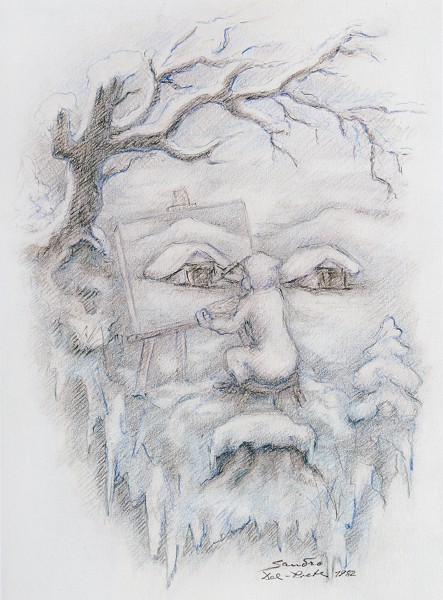
\includegraphics[width=0.99\textwidth]{sdp_mountain_spirit.jpg}
    \caption[Mountain Spirit in Winter by Snadro del Prete]{Mountain Spirit in Winter by Snadro del Prete. The image is from \citeay{sdp_mountain}.}
    \figlbl{sdp_mountain}
\end{figure}


\paragraph{Ambiguity.} Probabilistic neurons permits the persistence of multiple subnetworks, enabling the system to handle ambiguity effectively. For example, when presented with a composite face comprised of distinct objects (c.f. \figref{sdp_mountain}), both the subnetwork responsible for abstract faces and the subnetworks associated with individual objects become active concurrently. Consequently, one can attend to these subnetworks simultaneously, utilizing attention in its original sense rather than the conventional deep neural network (DNN) interpretation. I speculate that this represents a fundamental distinction from neural networks that are compelled to represent the entire scene within a single high-dimensional dense vector.

\paragraph{Interpretability.} The probabilistic frame allows for much better interpretability than classical deep networks. Each neuron can be part of a multitude of subnetworks and thus some semantic, i.e. corresponds to something meaningful. Furthermore, its internal state is a probability that can be interpreted as the networks confidence that this specific feature was observed in the input. A network of probabilistic neurons that support each other over timesteps can also be interpreted as a directed graph. This allows to trace how subnetworks are activated. Without formal proof or presenting an interpretability framework, I speculate that using this probabilistic framework will significantly simplify the explainability of intelligent systems.

\paragraph{Robustness.} A neural networks is usually represented with a vector which is sequentially processed by a mathematical functions (e.g. with neural layers). Artificial networks in particular are not robust to noise and are susceptible to adversarial attacks \sidecite{Akhtar_Mian_2018}. Slight changes to the input or a network-internal vector can completely falsify the overall result. This is because typical artificial networks work with continuous numbers and these feature vectors can consequently lie anywhere in the feature space. Therefore, a minimal change, e.g. triggered by noise, can shift the feature to the other side of the decision boundary and change the result. A binary vector, on the other hand, has different mathematical properties and is more robust against noise and adversarial attacks, especially if they are sparse and distributed\sidenote{only a small portion of the bits are ``on'', and representations differ by multiple binary bits} \sidecite{Ahmad_Hawkins_2015}.
Subsampled or noisy vectors are still semantically similar and are close to the original vectors when compared, for example by counting the overlap of bits between two vectors.

\section{Implementation}
TODO Add Overview of entire system


\subsection{Processing Loops}
The proposed framework introduces nested learning cycles, each with a different functionality. Since the proposed framework runs on a tacked computer hardware, the cycles are bound to fixed timesteps. At each timestep, the innermost loops executes a step. As soon as the innermost loop is finished, an outer loops takes a step and the process is repeated.

\begin{itemize}
\item[\textbf{Slow Loop}] The dataset comprises $D$ images, with each image depicting a randomly generated line. The images are processed one after the other, building the outermost loop.
\item[\textbf{Medium Loop}] For each image in $D$, $V$ different views are sampled by slightly changing the image. This generates $V$ distinct yet visually similar images. Similar to our visual system, which captures multiple frames of an object before moving on to the next, this loop allows to perceive objects from various viewpoints.
\item[\textbf{Fast Loop}] From each view $V$, a sensory system creates neural activity that is processed by the network for $T$ timesteps. This loop allows the network to build subnetworks over several timesteps. First, the network has a high neural activity, which is quickly reduced within these $T$ steps as only the activations with enough lateral support remain active and build an attractor state.
\end{itemize}



\subsection{Sensory Input}
An intelligent agent may have a multitude of sensory input. The main difficultly is that sensory input (especially images) are in continuous space, and they must be translated into an activation potential.
Thus, the sensory input must be linked to probabilistic neurons. Such a sensory system can be implemented by using either Gabor filters \sidecite{Gabor_1946, Granlund_1978} or, in a more advanced setting, with learned filters.
Such filters can be learned, for example, by training a deep network in a autoencoding setting \sidecite{rumelhart1985learning}. Even though such networks violate the principles from the Gestalt phenomena, their first layer exhibit excellent capabilities in extracting relevant features from images. Therefore, I argue that such filters are well suited as a network's sensory system if only the first layers are kept. However, also the output $\boldsymbol{h}$ of such as layer is not binary.
One option is to consider the normalized values of $\boldsymbol{h}$ as probabilities, with the notion that higher values indicate regions where a filter discovers matching features in the image. Alternatively, another approach involves setting all values in $\boldsymbol{h}$ above a pre-defined threshold to 1 and assigning 0 to the remaining values.
As a third option, quantization networks such as VQ-VAEs \sidecite{NIPS2017_7a98af17} can be used to map local features to a discrete value that can be translated in a binary activation pattern.

This thesis focuses on implementing a proof-of-concepts for handling straightforward images, which allows the utilization of a pre-defined hand-crafted sensory system. However, when processing complex natural images in future research, it is imperative to conduct empirical investigations to explore these possibilities further.

\subsection{Feature Extractor (L1)}
The sensory system converts an image into a binary observation of size $C_{in} \times W \times H$ where $C_{in}$ is the number of input channels, $W$ the image width and $H$ the image height. Thus, we have multiple cells representing one of $C_{in}$ feature at each pixel location. Let's denote a cell of feature channel $c \in \{0, ..., C_{in}\}$ at position $w \in \{0, ..., W\}$, $h \in \{0, ..., H\}$ as $x_{cwh}$. 





\subsection{Object Representation (L2)}



\subsection{L2 Grounding and Feedback}
TODO: Read this section and improve it!

This section explores the concept of grounding the activity of subnetworks into model representations within the model recognition layer (L2). L2 comprises abstract representations of various models, ideally invariant to transformations such as rotations or scaling. The mapping from the preceding layer to L2, facilitated by fibers, must handle the desired invariance to these transformations.

The objectives of this layer are twofold. Firstly, it serves as the component responsible for recognizing the objects perceived in the preceding layer. Secondly, it provides feedback to the preceding layer regarding the suitability of the representations or current subnetworks for successful recognition.

L2 also consists of probabilistic neurons that encode abstract representations of different objects. It is important to note that, in the long term, an object or concept can have multiple representations. For example, a face is an abstract construct comprising eyes, a nose, and a mouth, regardless of whether it is depicted on paper, encountered in the real world, or constructed from various objects. Thus, L2 should be capable of storing an invariant model of faces, enabling the recognition of faces regardless of how they are presented to L1.

The construction of L2 remains unclear. In humans, L2 is believed to possess substantial prior knowledge, which is refined based on the environmental experiences during childhood.

As an initial iteration, a fixed version of L2 can be created. Essentially, L2 needs to be modeled as a set of probabilistic neurons, and it may require joint development with L1 in a reciprocal process. However, we will begin by establishing a fixed representation for L2. For instance, when working with MNIST numbers, a binary code vector can be used to represent each object. These binary code representations can be learned using rigorous regularization techniques, thereby representing MNIST numbers as fixed neurons that are either active or inactive (i.e., with a probability of 1 or 0).

L2 is envisioned to serve not only in matching objects to invariant representations but also in providing feedback and reinforcement. If the representations in L1 successfully match a concept in L2 and exhibit minimal ambiguity (e.g., confidently identifying an image as a "7" rather than assigning similar probabilities to different numbers), they should be rewarded. This reward can be administered through neurotransmitters, thereby strengthening the connections among neurons within the subnetwork that recognized the object model stored in L2.

Consequently, two types of signals are employed to reinforce or weaken connections between neurons: co-activity and usefulness.













TODO: Neues Kapitel mit konkreter Implementierung: Basierend auf Overleaf Chapters "Connect to Sensory Inputs" und "Layer-2 Grounding and Feedback"


TODO: teste was passiert wenn Noise in Feature Extractor statt Image -> wird dieser entfernt?
TODO: Teste anderen Noise, z.B. Kreis
TODO: Kann das hire L2 sein: https://github.com/bacnguyencong/rbm-pytorch/blob/master/rbm.py? Wir minimieren die Energy Function zwischen verschiedenen Views (L1, =v_gibb) und Prototype (L2, =v)






